\documentclass[./main]{subfiles}

\begin{document}
  \chapter{A Toy Model: Sorting~Networks.}

  Here we use \textit{comparators}: a very small processor able to, given $a$ and $b$, sort the two numbers.
  Can we organize and connect comparators in order to sort a sequence of numbers?

  \begin{figure}[H]
    \centering
    \begin{tikzpicture}
      \draw (0, 0) rectangle (1, 1);
      \draw (-0.5, 0.25) -- (0, 0.25);
      \draw (-0.5, 0.75) -- (0, 0.75);
      \draw (1, 0.25) -- (1.5, 0.25);
      \draw (1, 0.75) -- (1.5, 0.75);
    \end{tikzpicture}
    \quad\quad\quad
    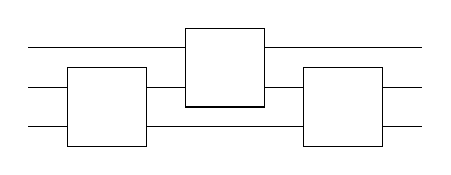
\begin{tikzpicture}
      \draw (0, 0) rectangle (1, 1);
      \draw (1.5, 0.5) rectangle (2.5, 1.5);
      \draw (3, 0) rectangle (4, 1);
      \draw (-0.5, 0.25) -- (0, 0.25);
      \draw (-0.5, 0.75) -- (0, 0.75);
      \draw (1, 0.25) -- (1.5, 0.25);
      \draw (1, 0.75) -- (1.5, 0.75);
      \draw (-0.5, 1.25) -- (1.5, 1.25);
      \draw (1, 0.25) -- (3, 0.25);
      \draw (2.5, 0.75) -- (3, 0.75);
      \draw (4, 0.25) -- (4.5, 0.25);
      \draw (4, 0.75) -- (4.5, 0.75);
      \draw (2.5, 1.25) -- (4.5, 1.25);
    \end{tikzpicture}
    %% --+-----+---
    %%   |     |
    %% --+-\ /-+-+--
    %%      X    |
    %% --+-/ \-+-+--
    %%   |     |
    %% --+-----+----
    %% TODO
    \caption{Sorting networks for two, three and four numbers}
  \end{figure}

  Here we want to optimize in two ways: minimize the number of steps, and minimize the number of comparators.

  \section{Odd-Even merge sort.}

  The Odd-Even merge sort is a parallel algorithm very similar to merge sort: we start by sorting two halves and then merging the two.
  In this section, we will consider an input of size $n = 2^m$.

  \subsection{Odd-Even merging network.}

  Given a sequence $c = \langle c_1, c_2, \ldots, c_n \rangle$, we want to compute a sequence written $\mathsf{SORT}(\langle c_1, c_2, \ldots, c_n \rangle)$ which corresponds to the sorted sequence of the $c_i$'s.
  If a sequence $c$ is sorted, we write $\mathsf{SORTED}(\langle c_1, \ldots, c_n \rangle)$.
  
  An important part of the merge sort is the following:
  \begin{quote}
    if $\mathsf{SORTED}(\langle a_1, \ldots, a_n \rangle)$
    and $\mathsf{SORTED}(\langle b_1, \ldots, b_n \rangle)$
    then
    \begin{align*}
      \mathsf{MERGE}(\langle a_1, \ldots, a_n \rangle, &\langle b_1, \ldots, b_n \rangle)\\
    &= \mathsf{SORT}(\langle a_1, \ldots, a_n, b_1, \ldots, b_n \rangle)
    .\end{align*}
  \end{quote}

  Let $\mathsf{MERGE}_m$ be a network merging two sequences of size $n = 2^m$.


    %% --------+---
    %%         |
    %% ----\ /-+-+--
    %%      X    |
    %% ----/ \-+-+--
    %%         |
    %% --------+----
    %% TODO

\end{document}
